\documentclass[a4paper,12pt]{report}
\usepackage{graphicx}
\usepackage{array}
\graphicspath{{./images/}}
\begin{document}
	\begin{titlepage}
		\begin{center}
			
\includegraphics{ankara_bilim.png}
		\end{center}
		\vspace{1cm}
		\begin{center}
			\LARGE
			\textbf{SENG 244 - Object Oriented Software Engineering}
		\end{center}
		\vspace{1cm}
		\begin{center}
			\Large
			\textbf{Software Design Document}
		\end{center}
		\vspace{1cm}
		\begin{center}
			\Large
			\textbf{Non Governmental Organization - Aid Operations Management System}
		\end{center}
		\vspace{2cm}
		\begin{center}
			\large
			\textbf{BETG-4}
		\end{center}
		\vspace{1cm}
		\begin{center}
			\large
			Bora Eskin - 210201021\\
			Eren Demir Özalban - 220201031\\
			Talha Fatih Bülbül - 220204007\\
			Gürkan Köleoğlu - 200204043
		\end{center}
	\end{titlepage}
	
	\tableofcontents
	
	\chapter{Introduction}
		\section{Purpose of System}
  			\paragraph{}The NGO Aid Operations Management System (NGO-AOMSYS) is designed to streamline the process of managing aid provisions for Non-Governmental Organizations (NGOs).
     			\paragraph{}The system aims to efficiently allocate and distribute aid, both in-kind and in-cash, to indigent individuals and households in need.
	  		\paragraph{}By providing a platform for donors to contribute, volunteers to engage, and aid recipients to apply for assistance, NGO-AOMSYS aims to improve the overall effectiveness and transparency of aid operations.
		\section{Design Goals}
  			\paragraph{}Efficiency: Automate the process of donation collection, volunteer registration, and aid distribution to reduce manual effort and improve response time.
     			\paragraph{}Transparency: Provide donors, volunteers, and aid recipients with visibility into the aid allocation process, including tracking their contributions and assistance requests.
			\paragraph{}Scalability: Accommodate a growing number of users, donations, and aid requests without compromising system performance.
   			\paragraph{}Accessibility: Ensure that the system is user-friendly and accessible to individuals with varying levels of technical expertise.
		\section{Definitions, Acronyms and Abbreviations}
  			\paragraph{}Donor: An individual or organization that contributes funds or materials to the NGO-AOMSYS system.
     			\paragraph{}Volunteer: An individual who offers their time and services to support aid operations.
			\paragraph{}Indigent: Individuals or households in need of aid assistance.
   			\paragraph{}Geographic Information System (GIS): A system designed to capture, store, manipulate, analyze, manage, and present spatial or geographic data.
      			\paragraph{}In-kind: Non-monetary contributions such as goods, services, or materials.
	 		\paragraph{}In-cash: Monetary contributions.
    			\paragraph{}Work Breakdown Structure (WBS): A hierarchical decomposition of the total scope of work to be carried out by the project team.
		\section{References}
  			\paragraph{} NGO Coordination Resource Center. (2024). "Title." Access Date: [29/04/2024], Access Address: [https://ngocoordination.org/en/library/types/manual-toolkits-and-guidance].
		\section{Overview}
  			\paragraph{}This document provides a detailed description of the NGO Aid Operations Management System (NGO-AOMSYS) software design. It outlines the purpose of the system, design goals, definitions, acronyms, and abbreviations used. The document also includes a reference section listing sources of information. The subsequent sections of the document will delve into the system's architecture, functionality, user interface, database design, and other key aspects.
	\chapter{Current Software Architecture}
	\chapter{Proposed Software Architecture}
		\section{Overview}
			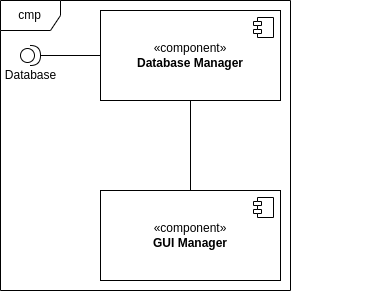
\includegraphics{component_diagram.png}
			\paragraph{}The product being developed is mainly made up of two components. The Database Manager and GUI Manager. Database Manager can be considered as the entire system of backend and GUI Manager the entire system of frontend. Database Manager, as the name implies, is responsible for managing the database. While the GUI Manager handles what to be shown to the user. 
		\section{Subsystem Decomposition}
			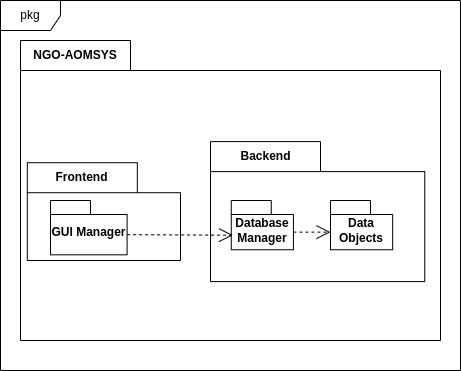
\includegraphics{subsystem_decomposition_diagram.png}
		\section{Hardware/Software Mapping}
		\section{Persistent Data Management}
		\section{Access Control and Security}
		\section{Boundary Conditions}
		\section{Subsystem Services Glossary}
	\chapter{Object Design}
		\section{Object Design Trade-Offs}
		\section{Interface Documentation Guidelines}
		\section{Packages}
		\section{Class Interfaces Glossary}
\end{document}
